% !TeX root = ../Book1.tex
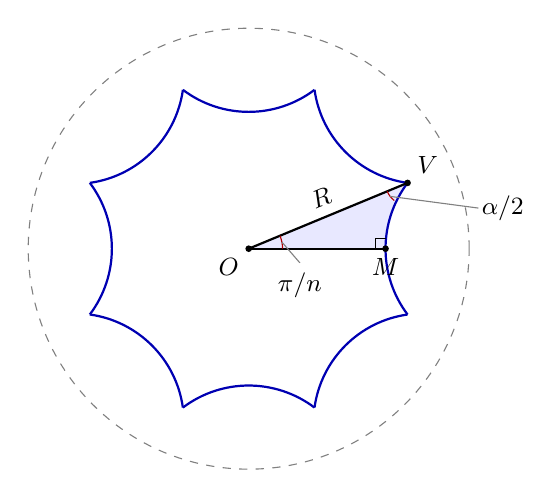
\begin{tikzpicture}[font=\small]
	\pgfmathsetmacro{\PlotRadius}{2.8}
	\pgfmathsetmacro{\VertexRadius}{.78}
	\pgfmathsetmacro{\HalfAngle}{22.5}
	\pgfmathsetmacro{\CircleCenter}{(1+\VertexRadius^2)/(2*\VertexRadius*cos(\HalfAngle))}
	\pgfmathsetmacro{\CircleRadius}{sqrt(\CircleCenter^2-1)}
	\pgfmathsetmacro{\ArcAngle}{atan2(\VertexRadius*sin(\HalfAngle),\CircleCenter-\VertexRadius*cos(\HalfAngle))}
	\pgfmathsetmacro{\Midpoint}{\PlotRadius*(\CircleCenter-\CircleRadius)}
	\coordinate (O) at (0,0);
	\coordinate (M) at (\Midpoint,0);
	\coordinate (V) at ({\PlotRadius*\VertexRadius*cos(\HalfAngle)},{\PlotRadius*\VertexRadius*sin(\HalfAngle)});
	\fill[blue!9] (O)--(M) arc[start angle=180,end angle={180-\ArcAngle},radius={\PlotRadius*\CircleRadius}]--cycle;
	\draw[dashed,gray] (O) circle (\PlotRadius);
	\foreach \j in {0,...,7}{
		\pgfmathsetmacro{\MiddleAngle}{45*\j}
		\draw[thick,blue!70!black] ({\PlotRadius*\VertexRadius*cos(\MiddleAngle-\HalfAngle)},{\PlotRadius*\VertexRadius*sin(\MiddleAngle-\HalfAngle)}) arc[start angle={\MiddleAngle+180+\ArcAngle},end angle={\MiddleAngle+180-\ArcAngle},radius={\PlotRadius*\CircleRadius}];
	}
	\draw[thick] (O)--(M);
	\draw[thick] (O)--node[midway,above,sloped] {\(R\)}(V);
	\draw (\Midpoint-.13,0)--(\Midpoint-.13,.13)--(\Midpoint,.13);
	\draw[red!70!black] (.43,0) arc[start angle=0,end angle=\HalfAngle,radius=.43];
	\node[below] at (.65,-.18) {\(\pi/n\)};
	\draw[thin,gray] (.65,-.18)--({.43*cos(\HalfAngle/2)},{.43*sin(\HalfAngle/2)});
	\begin{scope}[shift={(V)}]
		\draw[red!70!black] ({.28*cos(180+\HalfAngle)},{.28*sin(180+\HalfAngle)}) arc[start angle={180+\HalfAngle},end angle={270-\ArcAngle},radius=.28];
		\draw[thin,gray] ({.28*cos((450+\HalfAngle-\ArcAngle)/2)},{.28*sin((450+\HalfAngle-\ArcAngle)/2)})--(.9,-.32);
		\node[right,fill=white,inner sep=1pt] at (.9,-.32) {\(\alpha/2\)};
	\end{scope}
	\foreach \p in {O,M,V}{\fill (\p) circle (1.2pt);}
	\node[below left] at (O) {\(O\)};
	\node[below] at (M) {\(M\)};
	\node[above right] at (V) {\(V\)};
\end{tikzpicture}
